\documentclass[preprint]{revtex4-1}
\usepackage{graphicx}
\usepackage{epstopdf}
\usepackage{amsmath}
\usepackage{hyperref}
\usepackage{booktabs}
\usepackage{color}

\usepackage{SIunits}
\newcommand{\wstar}{-0.023}
\newcommand{\Qstar}{0.25}

\setlength{\tabcolsep}{10pt}

\newenvironment{sistema}%
  {\left\lbrace\begin{array}{@{}l@{}}}%
  {\end{array}\right.}


\begin{document}
\title{Roles of icosahedral and crystal-like order \\ in hard spheres glass transition} 
%\title{Role of structural heterogeneity of the supercooled liquid\\ in the crystallization of hard spheres}
%\title{On the origin of polymorphism during the nucleation of hard spheres}
%\title{On the origin of crystal polymorphism in hard spheres}
%\title{Selection principle of polymorphs upon crystallization \\ in hard spheres}
%\title{Role of orientational order in the crystallization of hard spheres}
%\title{On the microscopic mechanism of crystallization in hard spheres:\\ role of bond
%orientational ordering}
%\title{Crystal Polymorphism starts before crystallization}
%\title{Crystal Polymorphism starts before crystallization}
%\title{Crystal Polymorphism before crystallization}


\author{Mathieu Leocmach} 

\author{Hajime Tanaka \footnote{E-mail: tanaka@iis.u-tokyo.ac.jp}} 
\affiliation{ {Institute of Industrial Science, University of Tokyo, 4-6-1 Komaba, Meguro-ku, Tokyo 153-8505, Japan} }

\date{Received September 27, 2011}

\begin{abstract}
\textbf{
A link between structural ordering and slow dynamics has recently attracted much attention from the context of the origin of glassy slow dynamics~\citep{cavagna2009supercooled,BerthierR}. There have been a few candidates for such structural order, icosahedral order~\cite{steinhardt1983boo,sadoc1999geometrical, tarjus2005fba}, exotic amorphous order~\cite{lubchenko2007}, and crystal-like order~\cite{tanaka2010critical}. Each type of order is linked to a different scenario of glass transition. Here we experimentally access local structural order in polydisperse hard spheres by its particle-level observation with confocal microscopy. We identify the key structures as icosahedral and face-centred-cubic(\textmd{\textsc{fcc}})-like order, excluding any other simple local symmetry. We find that both types of order are statistically associated with slow particles. However, when approaching the glass transition, the icosahedral order does not grow in size whereas crystal-like structures grow. It is the latter that governs the dynamics and is linked to dynamic heterogeneity. This questions the direct roles of the `local' icosahedral ordering in glassy slow dynamics and suggests that the growing lengthscale of structural order is essential for the slowing down of dynamics and the nonlocal cooperativity in particle motion. 
}
\end{abstract}
\maketitle



%The possibility of a non-crystalline order has been discussed mainly in relation to the long standing problem of the glass transition. Even %so, its role remains unclear: actively slowing down the system or avoiding crystal formation. This issue may be crucial in the design of good %glass formers.

Upon cooling, a liquid usually undergoes a first order transition to an ordered ground state (crystal or quasi-crystal). However, it is generally possible to avoid the transition and to form a metastable supercooled liquid. Upon further cooling the dynamics slows down dramatically by many orders of magnitude, leading to the impossibility to equilibrate the system in the experimental time scale below a temperature $T_g$ named the glass transition temperature. The nature of the glass transition (thermodynamic or kinetic, structural or purely dynamical) is still matter of debates after decades of intensive research (see~\citep{cavagna2009supercooled,BerthierR} for comprehensive reviews).

A part of the answer is believed to come from the dynamics in itself: a supercooled liquid is dynamically heterogeneous (see~\citep{BerthierR} for a review) and the characteristic size of the dynamical heterogeneity is growing when approaching the glass transition~\citep{yamamoto1998, Donati1999a}. The dynamical arrest may then be the analogue of the slowing down observed near a critical point when the characteristic size of the fluctuations diverges, although slowing down at a particle level is absent in ordinary critical phenomena. Here we note that the lengthscale defined by the dynamical heterogeneity is not static (one-time spatial correlation) but dynamic (two-time spatial correlation). 

In order to unveil static quantities, it is tempting to link dynamical heterogeneity to structural heterogeneity. Stable structures should move less than unstable ones.~\citet{Widmer-Cooper2005} demonstrated that the initial configuration of a simulation, independently of the initial dynamics, has a role in the heterogeneity of the dynamics. \citet{Berthier2007} pointed out later that this influence does not exist at the particle level, but on larger scales: medium-range particle configuration can be statistically linked to medium range dynamical heterogeneity. However these arguments are based on the iso-configurational ensemble (starting again and again simulations with different dynamics but with the same initial configuration), a method that has no experimental equivalent.

Given that a glass shows no long-range periodic order, structures different from a crystal, icosahedral  ~\cite{steinhardt1983boo,sadoc1999geometrical, tarjus2005fba} or amorphous order \cite{lubchenko2007}, are most often pointed as responsible for the dynamical arrest. Since the pioneering work of Frank, icosahedral order is the archetypal model of amorphous structures~\citep{Spaepen2000}. Locally, an icosahedron maximises the density of packing, but its five-fold symmetry is incompatible with long-range periodicity. Geometrical frustration associated with icosahedral ordering is proposed to be crucial for vitrification ~\cite{steinhardt1983boo,sadoc1999geometrical, tarjus2005fba}. It was also proposed that the percolation of icosahedral order is responsible for glass transition~\cite{Tomida1995}.  Evidence of icosahedral ordering has indeed been found in very dense hard sphere packings~\citep{Bernal1960, Clarke1993, Anikeenko2007, Malshe2011, Charbonneau}, in various simulation models~\citep{steinhardt1983boo, Tomida1995, Doye2003, Pedersen2010, Coslovich2011} and more recently in experimental dense metallic liquids~\citep{Reichert2000, Celino2007} and glasses~\citep{Luo2004, Wang2011}.

Icosahedral order (or more generally locally favoured structures of the liquid) plays a central role in the spin-glass-type theory~\cite{steinhardt1983boo} and the frustration-limited domain theory of the glass transition (see~\citep{tarjus2005fba} for a review). The former theory considers the icosahedral ordering under frustration. On the other hand, the latter theory takes as a reference state an unfrustrated icosahedral order existing in a curved space, even if (and because) this reference state is impossible to reach for the real system. If the space were curved, the locally preferred order of the liquid (icosahedral) would form a continuous ordered phase upon cooling. In the  euclidean space, however, this transition is avoided, yet the avoided transition temperature still acts as a critical point giving rise to diverging lengthscales (icosahedral domain size and defect size) that would explain the dynamical arrest. This theory suggests that the frustration-limited domains are the origin of the dynamical heterogeneity. Yet, to our knowledge, numerical systems where a link between icosahedral order and dynamical heterogeneity has been observed~\citep{Doye2003, Pedersen2010, Coslovich2011}, have a (quasi)crystalline ground state including icosahedra. Thus, icosahedra could be regarded as a structural motif linked to the crystalline ground state in these systems. From this point of view these results do not support the spin-glass or frustration-limited domain approaches, but rather the crystal-based approach (see below).

An alternative way of explaining the phenomenology of the glass transition is based on the structure of the crystal. Crystallisation, even if avoided, may have an influence on the supercooled fluid or the glass~\citep{TanakaGJPCM, Cavagna2003, VanMegen2009a} and is taken as a reference state. Simulations~\cite{tanaka2010critical, Pedersen2010, Coslovich2011} and experiments~\citep{tanaka2010critical} show that a local bond orientational order compatible with the ground state (crystal) symmetry does extend to medium range in several model supercooled systems. These transient but relatively stable structures seem to be correlated with the slow regions because they are low free-energy configurations. Furthermore, they lack extended positional order and thus could not be detected by macroscopic diffraction experiments. \textcolor{blue}{We emphasize that crystal-like bond orientational order is `not' crystal nuclei with solid nature, but transient medium-range structural order formed in a liquid (see below)}. 

In the present work, we focus on the colloidal (hard spheres) supercooled liquid \cite{pusey1987ogt} for two reasons. First, hard sphere-like colloidal particles can be tracked by confocal microscopy, giving access to the positions and dynamics of individual particles \cite{kegel2000swe, weeks2000}, thus allowing microscopic analysis of the dynamical and structural heterogeneity. \textcolor{blue}{Here we develop a new tracking method, which enables us to access not only the coordinate but also the size of a particle (see Methods and Supplementary Information (SI)). This allows us a detailed structural and dynamical analysis, which is not possible by conventional methods.}  Second, hard spheres have a well defined crystalline ground state of face-centred-cubic (\textsc{fcc}) or hexagonal-close-packed (\textsc{hcp}) symmetry and locally favoured structures of icosahedral symmetry. This allows us to distinguish the different scenarios of glass transition, in particular, the frustration-limited domain scenario, \textcolor{blue}{the amorphous order scenario}, and the medium range crystalline order scenario.



We were able to follow the volume fraction dependence of the dynamics over nearly three orders of magnitude (see Fig.~\ref{fig:vft}), confirming the basic phenomenology observed in experiments~\citep{pusey1987ogt, kegel2000swe, weeks2000, BerthierR} as well as simulations~\citep{tanaka2010critical} of similar systems: super-Arrhenius dependence of the structural relaxation time $\tau_\alpha$ upon $\phi$, that we fit by the Vogel-Fulcher-Tammann \textcolor{blue}{(VFT) law; non-Gaussianity of the dynamics, peaking at $t^{dh}(\phi)$, and dynamical heterogeneity of growing size $\xi_u$ (see SI for the definitions).} 



The local structures of our suspensions are identified by a detailed analysis of Steinhardt's bond orientational order (\textsc{boo})~\citep{steinhardt1983boo}, including original improvements (see Methods). Figure~\ref{fig:maps} summarizes our structure identification results. We find the distinctive signature of medium ranged crystalline order (\textsc{mrco}) of \textsc{fcc} type, without excluding some \textsc{hcp}. \textcolor{blue}{We stress that \textsc{mrco} does not correspond to crystal nucleus (see SI) and accompanies little increase in the local density.} We find no trace of \textsc{bcc}-like structure. As for the aperiodic structures, icosahedral order stands out without any other obvious rivals (Dodecahedron are present but can be considered as twisted icosahedron). \textcolor{blue}{Thus, we experimentally confirm the presence of the growing static order in polydisperse hard spheres, at odd with a recent work by Charbonneau et al. \cite{Charbonneau} 
(see SI for a possible origin of this discrepancy).} 



We establish that in our system the tendency towards icosahedral order is best monitored by $w_6$, whereas $Q_6$ is the natural crystal-like order parameter (see Methods for the definitions of $w_6$ and $Q_6$). The population of local structures in the $(w_6,Q_6)$-plane is shown in Fig.~\ref{fig:maps}c-d, which confirms that the two tendencies are present in the supercooled liquid of hard spheres. \textcolor{blue}{In particular icosahedra} are present even at a relatively low volume fraction (Fig.~\ref{fig:maps}d). Both tendencies become more pronounced for deeper supercooling (Fig.~\ref{fig:maps}c). Furthermore, Fig.~\ref{fig:maps}c shows clearly that icosahedral order and crystalline order are incompatible and frustrate one another.



In the introduction we mentioned the dynamic propensity invented by~\citet{Widmer-Cooper2005} as a trick only accessible via simulations. In our system, since we know the relevant structural order parameters ($w_6$ and $Q_6$), we can compute the square displacement of all the particles with the same initial local structure (iso-bond order ensemble) and call it \textcolor{blue}{\emph{bond order mobility}. We define the $w_6$-mobility as
\begin{equation}
	\Delta r^2(w_6, t) \equiv \left\langle \frac{
		\sum\limits_i{
			\left\|\vec{r_i}(t)-\vec{r_i}(0)\right\|^2 \delta(w_6^i-w_6)
			}
	}{
		\sum\limits_i{\delta(w_6^i-w_6)}
	}\right\rangle 
	\label{eq:bo_propensity}
\end{equation}
where the brackets denote ensemble averaging. $\Delta r^2(Q_6, t)$ and $\Delta r^2(w_6, Q_6, t)$ can be defined in the same way. 
The iso-configurational propensity is very powerful since it does not require any a priori information on structures and thus can probe any static order. This feature is absent in the \emph{bond order mobility}, but instead it has a merit that it is accessible even in a system that cannot be restarted \emph{ab libitum} from exactly the same overall configuration. In general the two quantities are not equivalent.}

Figure~\ref{fig:msd_Q6_w6} shows the bond order mobility (calculated at $t^{dh}$). Both structural order parameters have a clear correlation with the dynamics: the more structured is the environment, the more likely the particle will be slow. For all volume fractions, the mobility displays the same linear dependence upon $w_6$ (Fig.~\ref{fig:msd_Q6_w6}b). Once scaled by the mean square displacement all points collapse on the same line. This is not the case for the $Q_6$ dependence (Fig.~\ref{fig:msd_Q6_w6}c) which is more and more pronounced with increasing the degree of supercooling. In our most deeply supercooled sample, the crystal-like environments can be in average ten times slower than the bulk, whereas even the almost perfect icosahedra are in average only $40\%$ slower than the bulk. A complete screening of all the possible \textsc{boo} mobilities excludes any link between an other local symmetry (exotic amorphous order) and slow dynamics, at least in our system.

To explain our mobility data, we can refer to the cage picture, where a particle is considered as trapped in the cage formed by its neighbours. Once the particle has escaped from its cage, it is free to diffuse. In general, this picture is not correct due to dynamical heterogeneity, or nonlocal cooperativity of motion. In the case of the icosahedral environment, however, it seems to hold: the normalisation by the bulk \textsc{msd} takes into account the diffusion once out of the cage, and the remaining universal dependence upon $w_6$ holds the information about the ``quality'' of the cage. Efficient packing makes the 13 particles icosahedra more stable than a disordered structure. Thus the central particle has a low probability to escape from its cage and start diffusing. After cage escaping, however, it diffuses in average like any other particles. This suggests that the influence of icosahedral order on the dynamics is only local because of its isolated character. By contrast the non-trivial $\phi$ dependence of the $Q_6$-mobility calls for nonlocal explanations.

To observe the ordered regions in real space, we define the thresholds $w_6^*$ and $Q_6^*$ so that the bond order mobility at the threshold is half between the bulk and the (extrapolated) prefect structure. In our most deeply supercooled sample, this criterion yields $w_6^* = \wstar$ for icosahedral structures (see Fig. ~\ref{fig:3D}a) and $Q_6^* = \Qstar$ for crystal-like structures (see Fig. ~\ref{fig:3D}b). These thresholds are arbitrary but coherent with each another. We display in Fig.~\ref{fig:3D}c typical configurations of the ordered neighbourhoods in our deepest supercooled sample. With our thresholds, we see only small patches of icosahedral order that are not reaching medium range, whereas clusters of crystal-like order are much larger than icosahedral clusters and their sizes reach medium range. 



Consistently, we were not able to extract a lengthscale associated with the sole icosahedral order that would grow when approaching the glass transition. By contrast, the spatial extent of crystal-like order is well described by $G_6(r)$, the spatial correlation function of $Q_{6 m}$ (see, e.g., \cite{tanaka2010critical}). Both dynamical and structural lengthscales are increasing while approaching the glass transition in a coherent manner (the inset of Fig.~\ref{fig:vft}). We can see that the growth of both dynamic and static correlation length can be well expressed by the power law,   $\xi_{u,6} \propto (\phi/(\phi_0-\phi))^{-\nu}$ with $\nu=2/3$. In agreement with~\citep{tanaka2010critical} it suggests that the dynamical heterogeneity in hard spheres is a manifestation of critical-like fluctuations of the crystal-like bond orientational order parameter, and not those of icosahedral or amorphous order. In relation to this, we stress that $G_6(r)$ is constructed from the coarse-grained \textsc{boo} and thus not sensible to aperiodic structures such as icosahedral or amorphous order. 

Of course, one can set a more permissive threshold on $w_6$ and observe more icosahedra. A percolating network of icosahedral neighbourhood can even be found at a high volume fraction if the threshold encompasses enough particles. However, the imperfect icosahedra particles that must be included to form this network have a mobility comparable to the bulk (Fig.~\ref{fig:msd_Q6_w6}b). Furthermore, we checked that this percolation is of the 3D random percolation class (cluster size distribution follows a power-law of exponent $\approx 2.1$), meaning that a comparable network could be obtained by picking randomly the same number of particles. We conclude that the concept of icosahedral network is not physically meaningful in our system.

As a final but an intuitive check, we were able to compare the spatial repartition of stable crystal-like order (Fig.~\ref{fig:3D}d) and slow particles (Fig.~\ref{fig:3D}e). As shown in~\citep{Berthier2007}, the correlation between structure and dynamics is not a one-to-one correspondence at the particle level but a statistical relationship on larger length scales. We were able to show visually this correlation by averaging out short time ($t^{dh}/2$) fluctuations of $Q_6$; by calculating the square displacement of each particle over $2\tau_\alpha\approx 4.5t^{dh}$ which allow to accumulate many rearrangement events; and by coarse-graining this value over the particle's neighbours~\citep{Berthier2007} (see Eq.~(\ref{eq:Mu}) in Methods). Figure~\ref{fig:3D}e displays the $10\%$ slowest particles according to this criterion and their neighbours. The correlation of shape and size is clearly seen between Fig.~\ref{fig:3D}d and Fig.~\ref{fig:3D}e, although it is not perfect. The slight disagreement comes from the following reasons: some clusters of \textsc{fcc}-like order disappear soon after the initiation of the displacement measurement and some particle groups, which come back to their original positions after the period of $2\tau_\alpha$, can be accounted as slow particles. We note that no such correlation can be found between icosahedral particles (Fig.~\ref{fig:3D}c) and slow regions.



We have demonstrated that supercooled hard-sphere liquids display local icosahedral ordering while having structural ordering linked to the avoided crystalline (\textsc{fcc}) ground state. Both types of packing are efficient and thus locally favoured. Yet the icosahedral order remains local even at deep supercooling and (consistently with the arguments of~\citep{Berthier2007}) is not able to influence significantly the global dynamics. By contrast, the slowing down associated with the crystal-like symmetry is nonlocal and long-lived. The characteristic length scale of the crystal-like order grows when approaching the glass transition in the same way as the dynamical heterogeneity. This suggests that the structural origin of the dynamical arrest is linked to the avoided crystallisation and not to the condensation of the local (icosahedral) order of the liquid. We note that the development of structural order and its link to dynamic heterogeneity are at odds with purely kinetic scenarios of glass transition. 

For some systems, the first order transition avoided upon supercooling leads to a symmetry compatible with icosahedral order. The symmetry-breaking phase can be a quasi-crystal~\citep{Doye2003} or a Frank-Kasper crystal like recently demonstrated for Wahnstr\"om mixture~\citep{Pedersen2010}. In that case, the amorphous order cannot be distinguished from the defective crystalline order that slows down the system, so the amorphous order seems to play a role in the slowing down. However, we showed here that when the amorphous order is not compatible with the crystal symmetry, its role in the slowing down seems to be minor.

We do not say that the local (icosahedral) order of the liquid is unimportant in the glass transition. Actually it plays a role in preventing the first order transition (crystallisation) to happen, thus allowing supercooling and the glass transition \cite{TanakaMJPCM}. Furthermore, this frustration against crystallisation may be linked to the fragility of the glass former~\citep{TanakaGJPCM,tanaka2010critical}. Competing crystal-like and non-crystal-like orderings may be important in many glass-forming systems covering colloidal, molecular, polymeric, oxide, chalcogenide, and metallic glasses. In particular, our finding may have important implications on the physical mechanism responsible for the high glass-forming ability of bulk metallic glassformers~\cite{Wang2004}. 

\vspace{1cm}
\noindent
\textbf{Methods}

We used \textsc{pmma} (poly(methyl methacrylate)) colloids sterically stabilized with methacryloxypropyl terminated \textsc{pdms}(poly(dimethyl siloxane)) and fluorescently labelled with rhodamine isothiocyanate chemically bonded to the \textsc{pmma}. The size distribution, as characterised by scanning electron microscopy imaging, showed a long tail toward small sizes, leading to about $6\%$ polydispersity. This amount of polydispersity allows us to avoid \textcolor{blue}{or at least delay crystallisation~\cite{Zaccarelli2009} (crystallization monitoring method in SI)} but is too low for fractionation to happen~\citep{Fasolo2003}. The colloids were suspended in a solvent mixture of cis-decalin and cyclohexyl-bromide for both optical index and density matching. To screen any (weak) electrostatic interactions, we dissolved tetrabutylammonium bromide salt, to a concentration of \unit{300}{\nano\mole\per\liter}~\citep{royall2005}. The estimated Debye screening length is \unit{100}{\nano\metre}, well below the length scale of the colloids. To avoid errors due to the swelling of the particles, their size was measured in the same solvent by the following technique: short-ranged depletion attraction was induced by adding non-adsorbing polystyrene to a dilute suspension to drive particles into contact; the position of the first peak of the $g(r)$ gave the diameter $\sigma = \unit{3.356\pm0.03}{\micro\meter}$.

After careful shear melting, the samples are filled into square $\unit{500}{\micro\metre}$ capillaries (Vitrocom). The most deeply supercooled sample showed a slight indication of sedimentation even after careful density matching. To avoid this effect we used a thinner $\unit{100}{\micro\metre}\times\unit{1}{\milli\metre}$ cell. The data was collected on a Leica SP5 confocal microscope, using \unit{532}{\nano\meter} laser excitation. The temperature was controlled on both stage and objective lens, allowing a more precise density matching. Our polydisperse colloids were detected using a novel multi-scale algorithm \textcolor{blue}{based on the scale invariant feature transform~\cite{Lowe2004} (see SI on the details), which allows} us to retrieve both position and size of each particle with about $1\%$ precision. The large size of our colloids allows a comparable precision in position for both in-plane and out-of-plane coordinates. The particles are tracked in time to extract dynamical informations. Typically $\approx 5000$ trajectories can be followed over a few structural relaxation times.



\citet{steinhardt1983boo} defined the \textsc{boo} of the $\ell$-fold symmetry as a $2\ell+1$ vector:
\begin{equation}
	q_{\ell m}(i) = \frac{1}{N_i}\sum_{0}^{N_i} Y_{\ell m}(\theta(\vec r_{ij}),\phi(\vec r_{ij}))
	\label{eq:qlm}
\end{equation}
where the $Y_{\ell m}$ are spherical harmonics. In the analysis, one uses the spherical invariants defined as:
\begin{align}
	q_\ell =& \sqrt{\frac{4\pi}{2l+1} \sum_{m=-\ell}^{\ell} |q_{\ell m}|^2 }\label{eq:ql}\\
	w_\ell =& \sum_{m_1+m_2+m_3=0} 
			\left( \begin{array}{ccc}
				\ell & \ell & \ell \\
				m_1 & m_2 & m_3 
			\end{array} \right)
			q_{\ell m_1} q_{\ell m_2} q_{\ell m_3} \label{eq:wl}\\
	\hat{w}_\ell =& w_\ell{\left( \sum_{m=-\ell}^{\ell} |q_{\ell m}|^2 \right)}^{-\frac{3}{2}}
\end{align}
where the term in brackets is the Wigner 3-j symbol. Note that the popular~\citep{steinhardt1983boo,Lechner2008} $\hat{w}_\ell$ can show a large norm if its denominator (or $q_\ell$) has small values (particle with low $\ell$-fold symmetry). Therefore, we have used here mostly the unreduced $w_\ell$ that pulls clearly apart highly symmetric particles from the fluid distribution.

Following~\citet{Lechner2008}, one can coarse-grain the tensorial \textsc{boo} over the neighbours:
\begin{equation}
	Q_{\ell m}(i) = \frac{1}{N(i)+1}\left( q_{\ell m}(i) +  \sum_{j=0}^{N(i)} q_{\ell m}(j)\right) 
	\label{eq:Qlm}
\end{equation}
and define coarse-grained invariants $Q_\ell$ and $W_\ell$ in the same way as Eqs.~(\ref{eq:ql}) and (\ref{eq:wl}). Structures with some amount of periodicity (crystalline) are then much easier to tell apart~\citep{Lechner2008}. However, non-periodic structures like icosahedra see their $Q_\ell$ and $W_\ell$ buried into the liquid distribution. With this in mind, we looked for periodic structures in the $\lbrace Q_\ell, W_\ell\rbrace$ space, and for aperiodic structures in the $\lbrace q_\ell, w_\ell\rbrace$ space, with $\ell=4,6,8,10$.

In both Eqs.~(\ref{eq:qlm}) and (\ref{eq:Qlm}), the sum runs over the ``neighbours'' of particle $i$. The definition of the neighbours is crucial for the consistency of the analysis. The most popular criterion in literature is that particles closer than $R_{max}$ are neighbours, with $R_{max}$ often fixed at the first minimum of $g(r)$. However, we find that this criterion has two major drawbacks: no account of polydispersity and negative correlation between the number of neighbours and the value of the $q_\ell$ (this effect is less pronounced after coarse-graining). To account for the polydispersity, we used a threshold in the scaled distance $\hat{r}_{i j} = r_{i j} /(\sigma_i+\sigma_j) < \hat{R}_{max}$, with $\hat{R}_{max}$ corresponding to the first minimum of $g(\hat{r})$. This allows us to look for structures without assumptions on the number of neighbours. 

We made a first round of analysis using this threshold definition, constructing maps similar to Fig.~\ref{fig:maps} but nosier. These maps allowed us to discard the possibility of \textsc{bcc} (high $Q_6$, low $Q_4$, high $Q_{10}$) and generally any structure except \textsc{fcc} (high $Q_6$, high $Q_4$ and $W_4<0$), \textsc{hcp} (high $Q_6$ and $W_4>0$) or icosahedron (very negative $w_6$, high $q_6$ and $q_{10}$). Dodecahedron can be found for $w_6>w_6^{dod}\approx -0.00782$, \emph{i.e.}, between the liquid and the icosahedral order. We are thus left with structures where the particles naturally have 12 neighbours. We then took a new \textsc{boo} analysis, this time taking the first 12 closest particles (in $\hat{r}$) as neighbours. This criterion reduces the noise in the distribution of the invariants and makes detected structures more easily comparable with crystallographic archetypes. It also avoids artefacts near $R_{max}$ in the correlation functions. The figures presented here were constructed from this second round of analysis.

This second definition of the neighbours is used consistently in the coarse graining of the square displacements:
\begin{equation}
	\bar{\Delta r^2}_i(t) = \frac{1}{N(i)+1}\left( {\Delta r^2}_i(t) + \sum_{j=0}^{N(i)} {\Delta r^2}_j(t) \right) 
	\label{eq:Mu}
\end{equation}
where ${\Delta r^2}_i(t) = \left\|\vec{r_i}(t)-\vec{r_i}(0)\right\|^2$ and the neighbours are defined at initial time. Note that we recover the correlation between crystalline order and slowness by two independent methods: directly in the instantaneous \textsc{boo} space via the mobility on moderate times; and indirectly via the positions and shapes of the (short time averaged) ordered regions coherent with those of the slowest regions (on long times). In the former method, the quality of the statistics comes from ensemble averaging over many realisations of each structure. In the later method, it comes from both coarse graining and the length of the trajectories that allow to accumulate many rearrangement events.

%\bibliographystyle{apsrev4-1}
\bibliographystyle{naturemag3}
\bibliography{ico_dyn}

\vspace{2cm}
\noindent
\textbf{Acknowledgments}

\noindent
The authors thank Paddy Royall and John Russo for fruitful discussions. 
This work was partially supported by a grant-in-aid from the 
Ministry of Education, Culture, Sports, Science and Technology, Japan. 

\sloppy
\noindent
{\bf Author Information} 
The authors declare that they have no competing financial interests. 
Correspondence and requests for materials should be addressed to 
H. T. 

\clearpage

\begin{figure}
\begin{center}
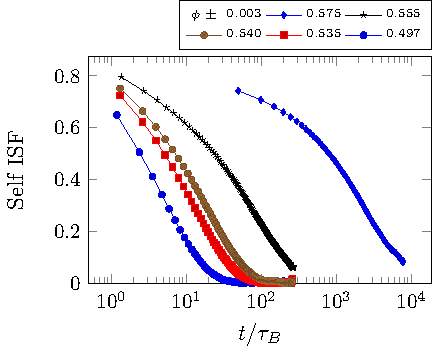
\includegraphics{generate_figures-figure0.pdf}
\end{center}
\caption{\textbf{Dynamics of the system.} {\bf a,} Decay of the self-intermediate scattering function computed from the positions for several volume fractions. {\bf b,} The structural relaxation time $\tau_\alpha$ and the characteristic time of the dynamic heterogeneity $t^{dh}$ scaled by the Brownian time $\tau_B$ as a function of $\phi$. The solid curve is the VFT fit of $\tau_\alpha$. Inset: Dynamical ($\xi_u$) and structural correlation length ($\xi_6$). Solid curves are power-law fits (see text).}
	\label{fig:vft}
\end{figure}

\clearpage

\begin{figure}
\begin{center}
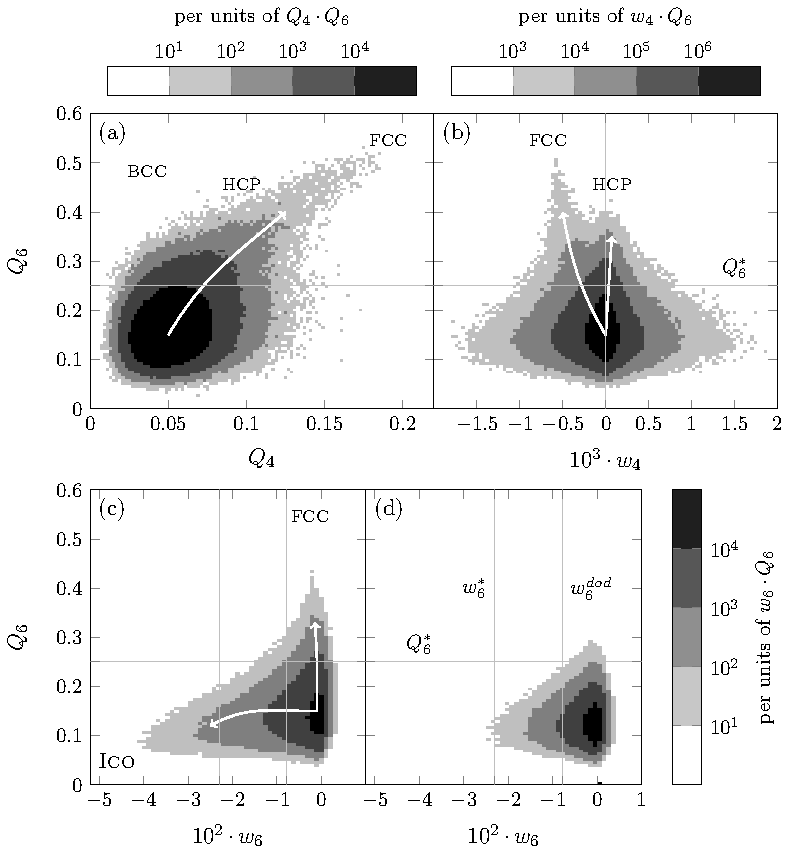
\includegraphics{generate_figures-figure1.pdf}
\end{center}
\caption{\textbf{Population of local structures function of the }\textsc{boo}\textbf{ parameters}. The values of \textsc{boo} parameters for a perfect structure are indicated by its name's position on each map. {\bf a-c,} For our deepest supercooled sample ($\phi=0.575\pm 0.03$) in the $(Q_4,Q_6)$-plane ({\bf a}), $(w_4,Q_6)$-plane ({\bf b}) and $(w_6,Q_6)$-plane ({\bf c}). {\bf d,} The same as {\bf c} but for a liquid near the freezing point ($\phi = 0.497 \pm 0.003$). Colour represents the probability to find the structure (log scale). The arrows stress the ordering tendencies: the tendency towards \textsc{fcc} is always visible, a weak tendency towards \textsc{hcp} can also be distinguished in {\bf b}, and the tendency towards icosahedral order is visible in {\bf c}.}
	\label{fig:maps}
\end{figure}

\clearpage

\begin{figure}
\begin{center}
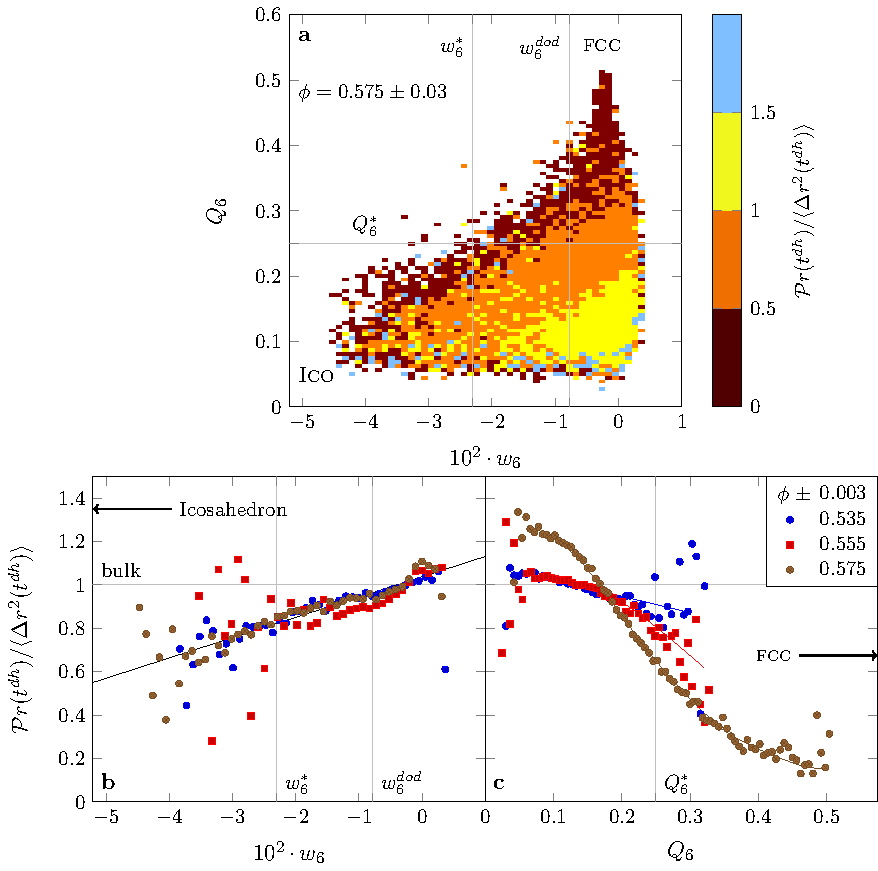
\includegraphics{generate_figures-figure2.pdf}
\end{center}
\caption{\textbf{Bond order mobility.} {\bf a,} Normalised mobility in the $(w_6, Q_6)$-plane for our most deeply supercooled sample. The colour scale is saturated at $1.5$ times the bulk mean square displacement. {\bf b-c,} Normalised mobility for icosahedral and crystalline order parameters respectively. Bulk mean square displacement is scaled to be at 1. Perfect structures are on the edge of each plot. The lines are a guide for the eye, stressing the collapse of the $w_6$-mobility at all volume fractions in {\bf b} and the absence of collapse in {\bf c}. The scattering at low volume fractions is due to poor averaging of rare structures.}
	\label{fig:msd_Q6_w6}
\end{figure}

\clearpage

\begin{figure}
\begin{center}
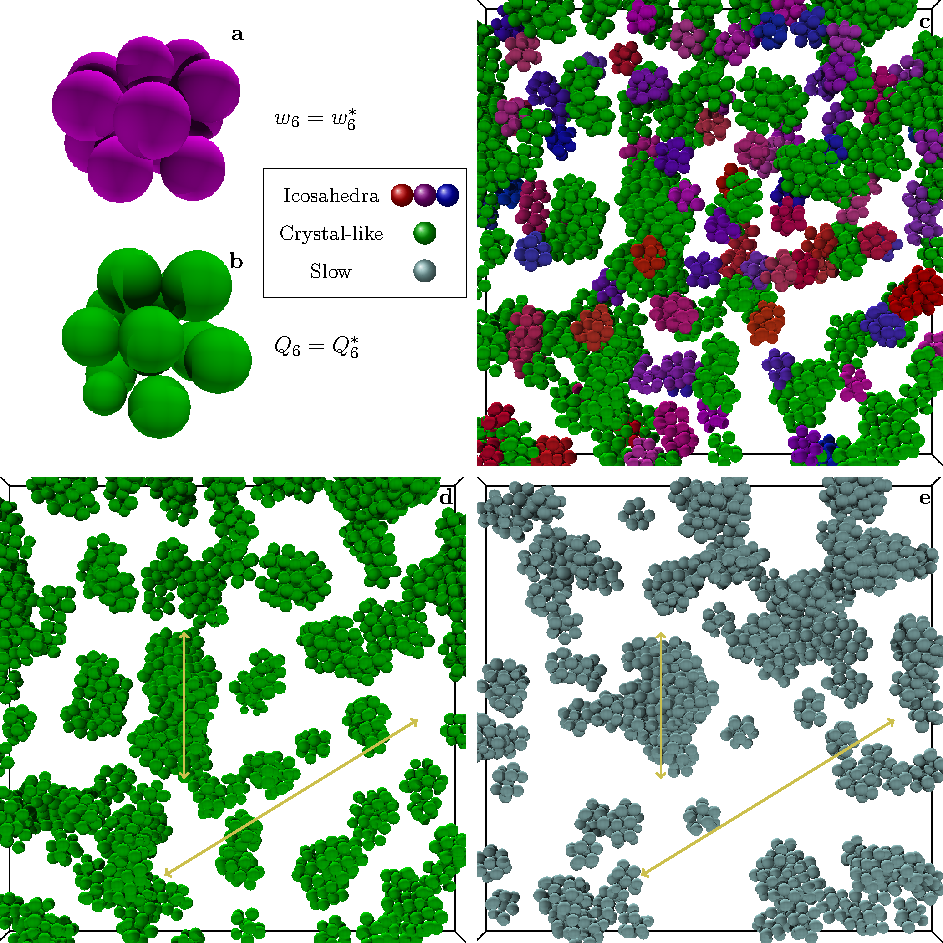
\includegraphics{generate_figures-figure3.pdf}
\end{center}
\caption{\textbf{Computer reconstruction from confocal microscopy coordinates in our most deeply supercooled sample.} Depth is $\sim 12\sigma$. Only particles of interest and their neighbours are displayed. Each particle is plotted with its real radius.  Example of \textbf{a} distorted icosahedron and \textbf{b} crystal-like cluster at the respective threshold values. \textbf{c,} A typical configuration of bond ordered particles. Two icosahedral particle are shown in the same shade if they belong to the same cluster. If a particle is neighbouring both kind of structures, it is displayed as icosahedral. \textbf{d,} Crystal-like particles alone (the order parameter was averaged over $t^{dh}/2$). \textbf{e,} Slow particles (see text). Due to particles going in and out of the field of view, the edges of \textbf{d} and \textbf{e} were not accurate and have been removed.}
	\label{fig:3D}
\end{figure}
\clearpage
\section*{Supplementary information}

\subsection*{Particle localisation and sizing}

Particle-level confocal microscopy experiments usually access the coordinates of the particles via the algorithm proposed by \citet{Crocker1996}. The original noisy image is blurred by convolution with a Gaussian kernel of width $\sigma$ to yield a soft peak per particle. Local intensity maxima within this blurred image give the coordinates of the particles with pixel resolution. Sub-pixel resolution ($0.1~0.3$~pixels error) can be achieved by taking the center of mass of a neighbourhood around the local maxima. The extension of this algorithm in 3D has been done in two ways: either tracking particles in each confocal plane and reconstructing the results (2D-flavour), or full image analysis on three dimensional pictures (3D-flavour).

The choice of the width $\sigma$ of the blurring kernel is critical: too small and the intensity profile is flat near the center of a particle, leading to multiple and ill-localized maxima per particle; too large and the peaks of nearby particles overlap, leading to shifts in the detected positions, or even fusion of the particles (only one particle detected instead of two). If the colloids are fairly monodisperse one can argue (at least in the 3D-flavour) that a range of possible width exist where the choice of $\sigma$ has almost no effect on the number of particle detected. Choosing $\sigma$ within this range gives confidence in the localisation results.

However, we found that no such ``good blur width'' exists in our $6\%$~polydisperse sample (see Fig.~\ref{fig:localise}c-h). The detection of smaller particles fails for blurring widths too small to detect properly the larger particles. This unacceptable failure of the \citet{Crocker1996} algorithm, as well as the want of the particles' radii data, triggered our design of a localisation algorithm that would be robust in the polydisperse case. Here we briefly disclose our method, leaving full details to a future publication.

The key notion to detect objects of unknown an possibly diverse sizes in an image is the \emph{scale space}~\cite{Lindeberg1993}. A popular implementation for isotropic objects (or ``blobs'') is the Scale Invariant Feature Transform (\textsc{sift}) of \citet{Lowe2004}. It consist in blurring the image by Gaussian kernels of logarithmically increasing widths ($\sigma_{i+1} = 2^{1/n} \sigma_i$, with $n$ a fixed integer, $n=3$ being a good choice) and taking the difference between consecutive blurred images. The difference of Gaussians (DoG) response function defined in this way depends on the position in space and on the scale. Bright objects in the original image are detected as local minima of the DoG in both space and scale, thus localisation \emph{and size} are determined simultaneously, without any assumption on the target size (see Fig.~\ref{fig:localise}a).

The \textsc{sift} is often used to match between different images complex objects consisting of many rigidly linked blobs further characterised by local histograms. To our knowledge, this method was never used for the quantitative localisation and sizing of independent single-blob objects like spherical colloids. The object-by-object optimal scale determination allows us to perform the spatial sub-pixel resolution step for each object on an image that is blurred just enough to have neither a flat intensity profile nor nearby peak overlap. This leads to a spatial resolution below $0.3$~pixels when two $10$-pixels wide particles are at hard-core contact, and less than $0.03$~pixels error ($0.3\%$ of the diameter) when any other particle's surface is further that $1$~pixel from the surface of the particle of interest.

At infinite dilution the scale $\sigma$ is simply proportional to the radius $R$ of the particle. Assuming a binary ball object, one finds
\begin{equation}
	R = \sigma \sqrt{\frac{3 \log 2}{n(1-2^{-2/n})}}
	\label{eq:scale_dil}
\end{equation}
We found that the radius of an isolated pixelated ball can be indeed measured within $0.3\%$ relative error with this method, provided a sub-scale resolution step similar to the spatial sub-pixel resolution step.

In dense suspensions, the neighbouring particles influence the scale dependence of DoG response. This effectively shifts the minima of the DoG toward smaller scales, leading to smaller radii if one uses Eq.~\ref{eq:scale_dil} alone. Assuming once again binary ball objects, one can take this coupling into account and construct a $N\times N$ system, with $N$ the number of particles, whose solutions are the radii and whose coefficients depend on the inter-particle distances. This system is actually very sparse (less than two dozen non-zero coefficients per line, even in the dense suspensions studied here) and the results converges in about two iterations. We measured the error in the resulting radii to be around $1\%$.

Recently \citet{Kurita2011,Kurita2011b} have designed a sizing method using particle coordinates from confocal experiments. However their method relies on coordinates extracted via the \citet{Crocker1996} algorithm which is defective when the size distribution is too broad, as described above. It may be possible to combine the two methods by feeding our coordinates and size as input to their method. We would expect an increase in sizing precision when the particles are close to contact.

\subsection*{Dynamics}

In Fig.~\ref{fig:vft}a we fit the self intermediate scattering function by the VFT law $\tau_\alpha=\tau_\alpha^0 \exp(D\phi/(\phi_0-\phi))$ ($D$ is the fragility index) to get the structural relaxation time $\tau_\alpha$ upon $\phi$. The non-Gaussianity of the dynamics is monitored by the kurtosis of the distribution of the displacements 
\begin{equation}
	\alpha_2(t) = \frac{3 \left\langle {\Delta r}^4(t) \right\rangle}{5 {\left\langle {\Delta r}^2(t) \right\rangle}^2}-1
	\label{eq:ng}
\end{equation}
At a given volume fraction, $\alpha_2(t)$ peaks at the characteristic time scale of the dynamic heterogeneity $t^{dh}(\phi)$. The volume fraction dependence of both $\tau_\alpha$ and $t^{dh}$ is plotted in Fig.~\ref{fig:vft}b. We notice that $t^{dh}$ corresponds to the end of plateau, always shorter than $\tau_\alpha$.

To define the characteristic length scale of the dynamic heterogeneity, we compute the mobility-mobility spatial correlation function~\cite{Donati1999}
\begin{equation}
	\mathcal{G}_u(r,t) = \frac{
		\left\langle \sum_{i,j}{\delta u_i(t) \delta u_j(t) \delta(r_{ij} -r)} \right\rangle 
	}{
		\left\langle \sum_{i,j}{\delta(r_{ij} -r)} \right\rangle
	}
	\label{eq:mobility_correl}
\end{equation}
which is a kind of four-point correlation function~\cite{cavagna2009supercooled}. The length scale $\xi_u$ is given by the fit of the envelope of $\mathcal{G}_u(r,t^{dh})$ in real space, at the characteristic time of the dynamic heterogeneity, by Orstein-Zernike form $\propto r^{-1}\exp( -r/\xi_u)$.

\subsection*{Difference between {\sc mrco} and crystal nuclei}

To avoid any confusion between our imperfect crystal-like order and well-formed but small crystals, we detect crystal nuclei \emph{via} the most standard method in the literature~\cite{ReintenWolde1996, Zaccarelli2009}. For each neighbouring particle, we compute the normalized scalar product of the (non coarse-grained) $q_{6 m}$:
\begin{equation}
	s(i,j) = \frac{
		\sum_{m=-6}^{6} q_{6 m}(i) q_{6 m}^{*}(j)
	}{
		\sqrt{\sum_{m=-6}^{6} |q_{6 m}(i)|^2} \sqrt{\sum_{m=-6}^{6} |q_{6 m}(j)|^2}
	}
	\label{eq:boo_dot_product}
\end{equation}
The bond between particles $i$ and $j$ is considered crystalline if $s_{ij}>0.7$~\cite{Zaccarelli2009}. A particle is crystalline if more than half of its bonds ($\geq 7$) are crystalline. 

Our small amount of polydispersity do not systematically prevent crystallisation~\cite{Zaccarelli2009}, thus we had to discard samples that append to crystallise. We find no large crystal nucleus in the samples analysed in the text. Even at deep supercooling a crystal nucleus never gathers more than 8 particles, and in total truly crystalline particles account for less than $1\%$ of the system. Fig.~\ref{fig:X_3D} compares the spatial extent of crystal nuclei and of the crystal-like clusters. Nuclei are systematically embedded into much larger \textsc{mrco}. One can explain this phenomenon as perfect wetting of the nuclei by coherently bond-ordered regions. However, examples of crystal-like structures without an embedded crystal nucleus, in addition to the continuity of $Q_6$ values (Fig.~\ref{fig:maps}), rather suggests that the crystal nuclei are the extreme part of the bond order fluctuations. In any case, trivial crystallisation cannot be responsible for the spatial extent of the dynamical heterogeneities (see Fig.~\ref{fig:3D}a and Fig.~\ref{fig:X_3D}e).

\subsection*{Bond order spatial correlation}

We used the same definition as in~\cite{tanaka2010critical} for coarse-grained bond order correlation function
\begin{equation}
	G_6(r) = \frac{4\pi}{13}\frac{\sum_{i,j} \sum_{m=-6}^{6} Q_{6 m}(i) Q_{6 m}^{*}(j) \delta(r_{ij}-r)}{\sum_{i,j} \delta(r_{ij}-r)}
	\label{eq:G_6}
\end{equation}
which is not sensible to the aperiodic structures. The envelope of $G_6(r)$ is fitted by Orstein-Zernike form to extract the crystal-like order correlation length $\xi_6$.

We stress that the correlation function defined by \citet{steinhardt1983boo} and used by \citet{Charbonneau} is correlating non-coarse-grained $q_{\ell m}$ and would be called $g_6(r)$ within our notation. As a consequence, it is sensible to crystal-like (slightly periodic) and icosahedral (aperiodic) order. We have seen in the main text that the first type of order reaches medium range where the second is not. However on the non-coarse-grained $q_6$ axis icosahedra stand out with the stronger signal and thus dominate the correlation measured by $g_6(r)$, making is appear short range and not growing. We think that this technical argument explains why \citet{Charbonneau} are not finding growing bond order lengthscale in their polydisperse ($8.5\%$) hard sphere simulations.

In addition, the symmetry-breaking phase of the binary hard sphere mixture of~\citep{Charbonneau} is not known and could possibly be not 6-fold symmetric. This would explain, in a coherent way with the main point of the main text, why 6-fold bond order parameters and correlation functions are not detecting growing static order. Indeed, the study of \textsc{boo} in binary systems is more problematic, as reported in~\citep{tanaka2010critical} for 2D binary soft disk simulations.

\clearpage

\begin{figure}
\begin{center}
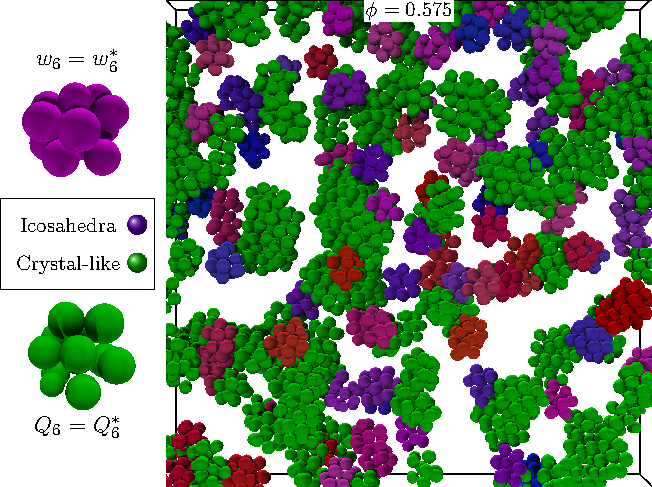
\includegraphics{generate_figures-figure5.pdf}
\end{center}
\caption{\textbf{Visualisation of the results of various tracking methods for the same portion of image.} \textbf{a} Multiscale 3D tracking. \textbf{b} Reconstruction from multiscale 2D tracking. \textbf{c-h} Crocker and Grier in 3D with blurring radius increasing from \unit{2}{px} to \unit{4.5}{px} by steps of \unit{0.5}{px}. The circles on each picture are the result of 2D multiscale tracking of each XY slice of the 3D pictures. Sphere are displayed with radii determined by the tracking methods in \textbf{a-b}, and equal to the blurring radius for \textbf{c-h}.}
	\label{fig:localise}
\end{figure}
\clearpage
\begin{figure}
\begin{center}
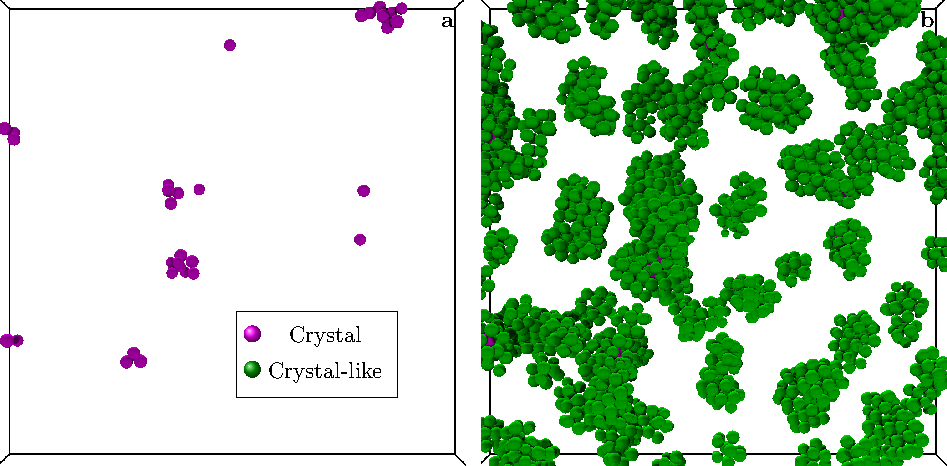
\includegraphics{generate_figures-figure4.pdf}
\end{center}
\caption{\textbf{Particles with more than $7$ crystalline bonds.} Particles with $Q_6>Q_6^*$ and their neighbours are also plotted in \textbf{b} for comparison. Crystalline particles are always included in high $Q_6$ regions. However, the fluctuations of the crystal-like order cannot be reduced to sub-critical nucleation.}
	\label{fig:X_3D}
\end{figure}

\end{document}